\documentclass[10pt]{article}
\usepackage[margin=1.2in]{geometry} % change page margin
\usepackage{graphicx} % display pictures
\usepackage{amsmath}  % math modes like 'align'
\usepackage{fancyvrb} % pretty spaces in verbatim
\usepackage{hyperref}

\title{POSIT, final report}
\author{
  Shay Agroskin \\
  \texttt{agroskinshay@campus.technion.ac.il}
  \and
  Shahaf Haller \\
  \texttt{hallershahaf@campus.technion.ac.il}
}


\begin{document}

\maketitle

\tableofcontents

\pagebreak

\section{Introduction}\label{sec:introduction}

The project analyzes a new way to do fractions arithmetic, instead of
the standard floating point implementation used today.

Fraction arithmetic efficiency and accuracy draws more attention in recent years
due to the growing popularity of machine learning and more complex graphic
designs (e.g.\ video games). While some approaches propose different
implementations of the current IEEE standard, other studies suggest a different
way to represent fractions all together.
This project studies one of these new formats called POSIT.

\subsection{Floating points}\label{sec:floatingpoints}

The current industry standard for fraction representation is the IEEE standard
754 (floats), in which a fraction is represented by three fields: sign, exponent
and significant. If we denote the sign as s, the exponent as e and significant
as f, then decimal representation of the number is:


\begin{align}
  {(-1)}^{s} \cdot 2^{e} \cdot f\label{eq:1} 
\end{align}

The range and precision of the numbers that can be represented using this format
depends on the number of bits used for the exponent and significant. The most
ubiquitously used lengths are a 32 bit vector, with 24 bits for the significant
part and a 64 bit vectors, with 53 bits for the significant part.

\begin{figure}[h]
  \centering
  \includegraphics*[width=\textwidth, height=1.5cm]{ieee_754_format}
  \caption{IEEE 754 standard fraction representation}\label{fig:ieee754}
\end{figure}

For example, the number 1.5 can be represented by setting $s=0, e=-2, f=6$ since
\begin{align*}
  {(-1)}^{0} \cdot 2^{-2} \cdot 6 = \frac{6}{4} = 1.5
\end{align*}

\subsection{Caveats}\label{sec:floatscaveats}

Although ubiquitous, the IEEE standard 754 has some several downsides. Since the
exponent and fraction bit lengths are fixed, the range and accuracy of a number
that can be represented using this format are limited, which in turn case some
problems.

\subsubsection{Representation problem}\label{sec:accuracyproblem}

The IEEE standard 754 requires choosing the base of the exponent part and the
number of bits to represent it during implementation. Regardless of the chosen
base, some number would always be impossible to represent exactly.

For example, by choosing base 2, the number $0.3$ cannot be represented
precisely and is rounded to a value that can be represented by
\begin{align*}
  {2}^{e}\cdot f
\end{align*}

Since $0.3$ representation is only and approximation of the real number, the
following Python code
\begin{verbatim}
> 0.3 + 0.3 + 0.3 == 0.9
\end{verbatim}
is mistakenly evaluated to ``False''.

\subsubsection{Granularity and Range problem}\label{sec:gran-range-probl}

The range and precision of an IEEE 754 number depend on the number of bits
allocated to it during implementation.
Allocating more bits to the exponent part can increase the precision of a
number, while increasing the significant field can increase its range.

As the number of bits is finite, one might choose a floating point
implementation where the precision and range match some of one's workflows but
not others. \ref{prec_value} shows the precision in two common implementations:
\begin{itemize}
  \item single precision-32 bit vector with 24 bits for the significant part
  \item double precision-64 bit vector with 53 bits for the significant part
\end{itemize}

\begin{figure}[h]
  \centering
  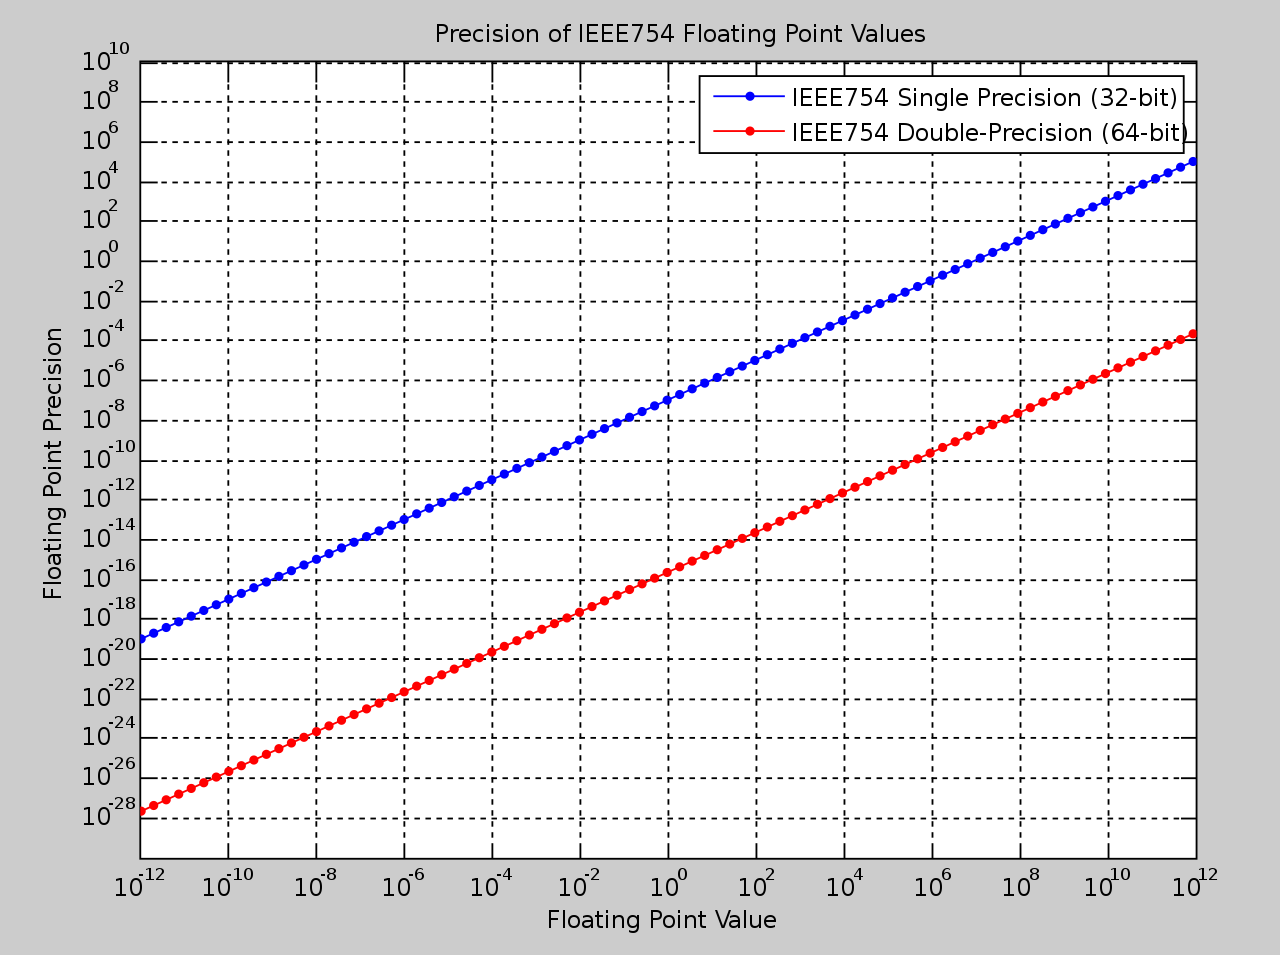
\includegraphics[width=\textwidth, height=0.3\paperheight]{1280px-IEEE754}
  \caption{Precision for different float values}\label{prec_value}
\end{figure}

\subsubsection{Wasteful representation}\label{sec:wast-repr}

There are more than one way to represent the same number using the existing
format. For example, the number 16 can be represented by
\begin{itemize}
  \item setting exponent part to zero and significant to 16 so that the number
    is ${2}^{0}\cdot 16$. Or
  \item setting the exponent part to 4 and significant to 1 so that the number
  is ${2}^{4} \cdot 1$
\end{itemize}

Moreover, in order to represent ``Not a number'' (NaN), an indication that the
result is invalid, the IEEE 754 format instruct to set all the exponent bits to
1. This results in a wasteful use of the significant bit, as any value of them,
combined with trailing ones in the exponent part would represent the same NaN.

\section{POSIT}\label{sec:posit}

In order to tackle some of the IEEE 754 format's problems, a new format was
proposed by John Gustavson which is called POSIT.

The new format divides the bit vector into four parts (\Ref{fig:posit_format}):
\textit{sign, regime, exponent} and \textit{fraction}, which together form the
decimal number:
\begin{align}
{(-1)}^{sign} \cdot ({useed}^{regime}) \cdot {2}^{exponent} \cdot 1.fraction \label{eq:2}
\end{align}

where $useed = 2^{2^{es}}$ and \textit{es} is the number of bits used for the exponent part.

\begin{figure}[h]
  \centering
  \includegraphics*[width=\textwidth]{POSIT_format}
  \caption{Generic posit format for finite, nonzero values}\label{fig:posit_format}
\end{figure}

\subsection{regime value}\label{sec:regime-value}

The \textit{regime} value depends on the running sequence starting after the sign bit in the
following manner:
\begin{align*}
  bbbbbbb\overline{b}
\end{align*}

in this sequence of n \textit{b}'s and one \textit{$\overline{b}$}
\begin{itemize}
  \item if b=0, the regime equals to -n
  \item if b=1, the regime equals to n-1
\end{itemize}

Figure \Ref{fig:regime_values} shows more examples of \textit{regime} sequences and their
value in the \Ref{eq:2} equation:

\begin{figure}[h]
  \centering
  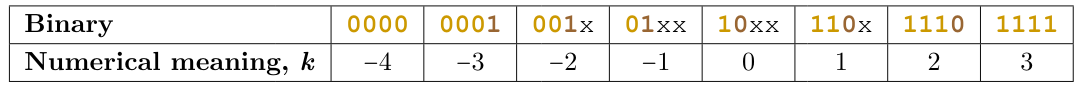
\includegraphics[width=\textwidth, height=0.04\paperheight]{regime_values}
  \caption{Different regime sequences and their respective value}\label{fig:regime_values}
\end{figure}


\subsection{Dynamic range and accuracy}\label{sec:dynam-range-accur}

As explain the \textit{regime} description \Ref{sec:regime-value}, the regime
field does not have a fixed size: The number of bits in the regime part are
determined by the first flipped bit after the bit sequence. \\\\
This implies that both \textit{01} and \textit{111111111111110} are valid regime sequences
(equal to $-1$ and $13$ respectively) which can be part of a 32bit POSIT vector.
In fact, the regime sequence can take up to the whole POSIT bit vector.
Since the exponent field size is fixed, the fraction bit width change according
the regime part.

If no flipped bit exists, meaning that the POSIT vector has to form of
\textit{$sbbbbbbbbb$} where \textit{s} is the sign bit, then the POSIT vector
receives a special value depending on the value of \textit{b} and \textit{s}
(see \autoref{sec:posit-speciel-values} for more information).

\paragraph{}
The dynamic field size help with the granularity and range problem
(\ref{sec:gran-range-probl}) by allowing workflows to use large regime
fields when working with very large number and small regime fields when in need
of high accuracy (the size of the fraction field is implied by the regime part).

\subsection{exponent and fraction fields}\label{sec:expon-fract-fields}

The \textit{exponent} field width, denoted as \textit{es}, is fixed and determined at
implementation. The field's starts after the first flipped bit that marks the
\textit{regime} field's end (see \autoref{sec:regime-value}). If there are less
than \textit{es} bits left after the \textit{regime} field, the
\textit{exponent} field is right-padded with zeroes.


\subsubsection{fraction field}\label{sec:fraction-field}
The \textit{fraction} part of the POSIT starts after the \textit{exponent} field
(see \autoref{fig:posit_format}) and its width depends on the number of bits
occupied by the \textit{sign}, \textit{regime} and \textit{exponent}
parts(\Ref{sec:regime-value}).

\paragraph{}
Unlike the IEEE 754 format, the POSIT format assumes that \textit{fraction} field only
describes the fractional part of a number $1\leq n < 2 $. For example, the
decimal representation of the \textit{fraction} field $b_{1},b_{2},\dots,b_{n}$
is:
\begin{align*}
 1 + \sum_{i=1}^{n}b_{i}\cdot 2^{-i}
\end{align*}

Combining the \textit{sign}, \textit{regime} and \textit{exponent} parts the
decimal representation of a POSIT vector is

\begin{align*}
{(-1)}^{sign} \cdot ({useed}^{regime}) \cdot {2}^{exponent} \cdot 1.fraction
\end{align*}

\autoref{fig:diff_posit_vals} shows different POSIT vectors and their decimal
value. As the figure shows, in case the fraction part is absent, it is assumed
to be zero (i.e. its decimal representation is $1 + 0 = 1$)

\begin{figure}[h]
  \centering
  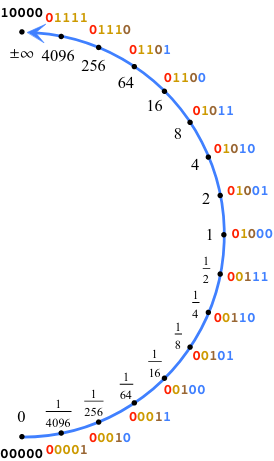
\includegraphics[height=0.25\paperheight]{posit_values}
  \caption{5-bit POSIT vectors with es = 2, useed = $2^{2^{es}} = 16$ and their
    decimal value}
  \label{fig:diff_posit_vals}
\end{figure}

\subsection{POSIT speciel values}\label{sec:posit-speciel-values}

POSIT format does not differentiate between $\pm\infty$ and represents them both
by setting the \textit{sign} bit and clearing the rest of the vector (as can be
seen in \autoref{fig:diff_posit_vals}). \\
Zero representation is a vector with all its bits cleared.

\paragraph{}
Unlike the IEEE 754 format, POSIT doesn't have a representation of NaN. In order
to signal that a computational result is invalid the hardware implementation of
the format should raise an interrupt.

\section{Related work}\label{sec:relatedwork}


One can calculate most of the fractions using rational representation

\subsection{Increasing Float size}\label{sec:increasefloat}

Over the years, the number of bits in floating point operations has
increased in order to imrpve number accuracy.


\end{document}

% LocalWords:  NaN
